%!TEX root = ./template-skripsi.tex

\subsection{\textit{Sprint 11}}

	\textit{Sprint-11} dilakukan sepekan pada tanggal 1 november 2022 sampai dengan 8 november 2022. \textit{Story} kesebelas pada \textit{product backlog} yaitu membuat fitur multiuser/login dan register dipecah menjadi beberapa \textit{task} sebagai berikut.


 \begin{longtable}[c]{@{} |p{1cm}|p{4cm}|p{5cm}|p{3cm}| @{}}
 \caption{\textit{Sprint 11} \label{sprint11_table}}\\


 \hline
  \multirow{1}{=}{\centering{\textbf{No}}} & \multirow{1}{=}{\centering{\textbf{\textit{Story}}}} & \multirow{1}{=}{\centering{\textbf{\textit{Task}}}} & \multirow{1}{=}{\centering{\textbf{\textit{Status}}}}\\
 \endfirsthead

 \hline
  \multirow{1}{=}{\centering{\textbf{No}}} & \multirow{1}{=}{\centering{\textbf{\textit{Story}}}} & \multirow{1}{=}{\centering{\textbf{\textit{Task}}}} & \multirow{1}{=}{\centering{\textbf{\textit{Status}}}}\\
 \endhead

 \hline
 \endfoot

 \hline
 \endlastfoot

 \hline
 1 & Membuat multiuser &  Membuat \textit{Mock-up UI} halaman login dan register &  selesai \\
 \hline
 2 & & Menerapkan \textit{Mock-up UI} halaman login dan register ke Flutter & selesai\\
 \hline
 3 & & Mengintegrasikan halaman login dan register ke \textit{webservice} & selesai\\
 \hline
 \end{longtable}

Pada sprint kesebelas ini story yang di pilih untuk di uraikan pada sprint kali ini adalah membuat login dan register. Tujuan dari \textit{sprint-11} ini adalah membuat multiuser dan mengintegrasikan halaman tersebut dengan webservice yang sudah dibuat oleh penelitian Andri Rahmanto.

\begin{enumerate}[listparindent=2em]
	
	\item{\textit{Membuat Mock-up UI Fitur multiuser}}
	
	Pembuatan konten dan fitur yang terdapat pada \textit{mock-up UI} fitur multiuser dilakukan berdasarkan persetujuan product owner dan scrum master pada meeting sebelumnya. Mock-up UI dibuat menggunakan platform figma.
	
	\begin{figure}[H]
	\centering
	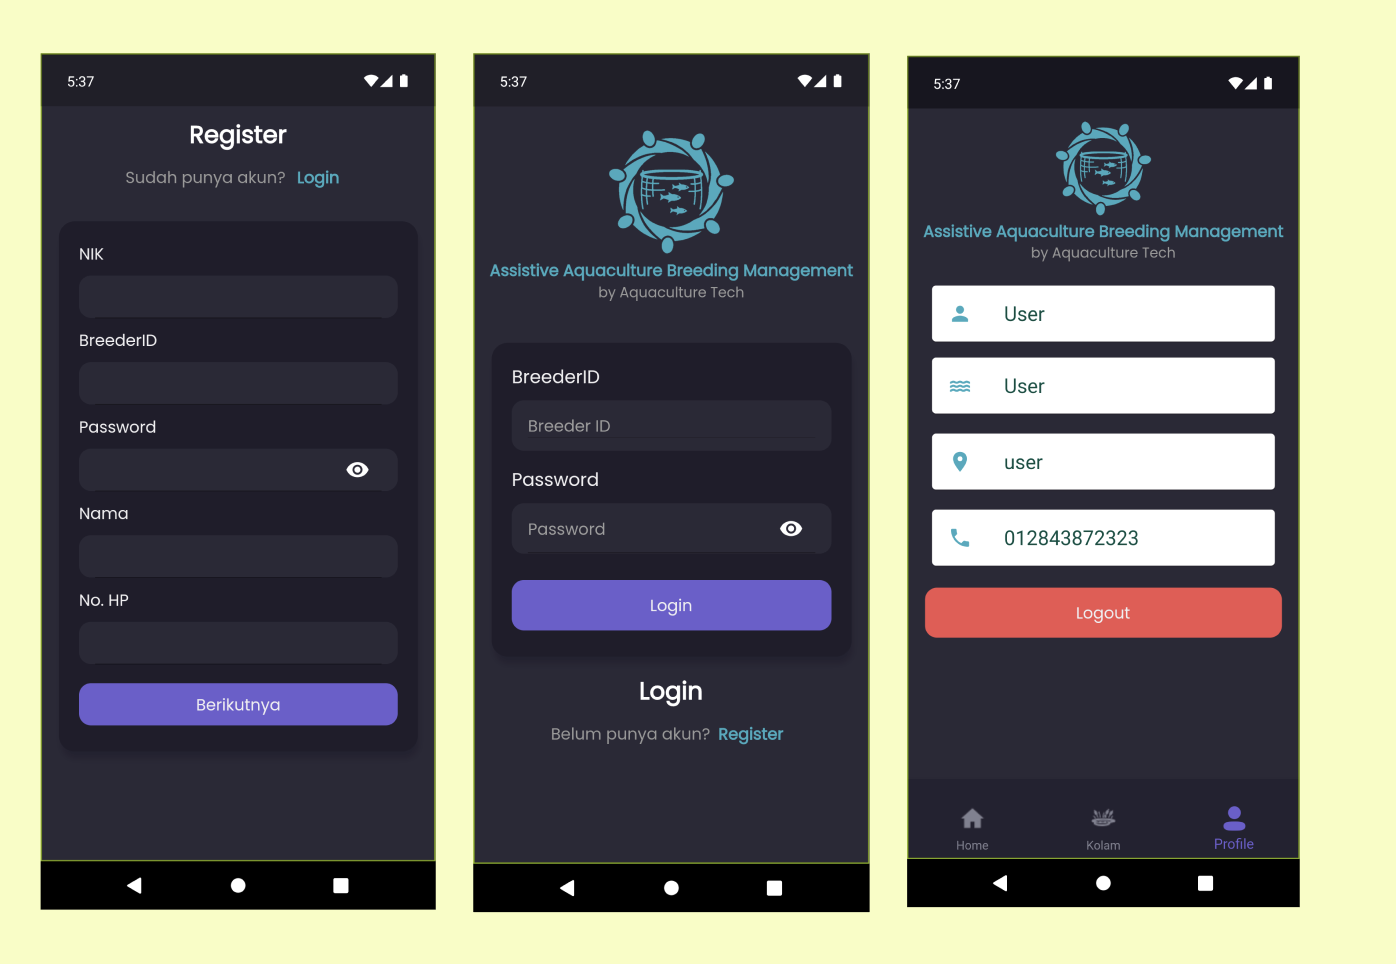
\includegraphics[keepaspectratio, width=6cm]{gambar/mockupmultiuser}
	\caption{\textit{Mock-up UI Fitur multiuser}}
	\label{gambar:mockupmultiuser}
	\end{figure}

	\item{\textit{Class Diagram}}
	
	Class Diagram menggambarkan kelas-kelas yang akan dipakai oleh sistem. Umumnya terdapat 3 kelas pada setiap module yaitu class model, controller, dan view. Pada sprint-11 penelitian kali ini penulis membuat 4 class yaitu model yang berwarna biru, view berwarna oranye, controller yang berwarna hijau, dan service yang berwarna kuning.
	 
	 \begin{figure}[H]
	 \centering
	 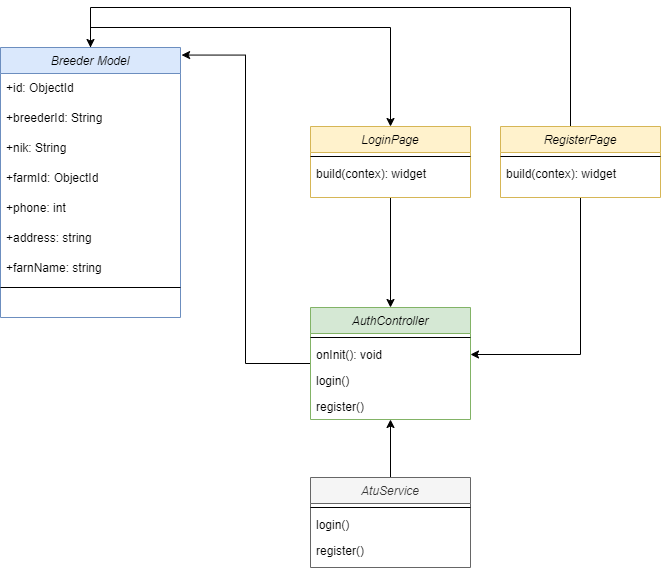
\includegraphics[keepaspectratio, width=6cm]{gambar/authcd}
	 \caption{\textit{Class Diagram Fitur Sprint-11}}
	 \label{gambar:authcd}
	 \end{figure}

	\item{\textit{Menerapkan Mockup-UI Fitur multiuser kedalam code flutter}}
	
	Setelah itu, akan dilakukan pengimplementasian \textit{mock-up UI} ke dalam aplikasi menggukan flutter. Pada lampiran 12 terdapat source code dari implementasi fitur multiuser yang dikelompokan berdasarkan halaman yang menghasilkan output halaman seperti pada gambar dibawah ini.

	\begin{figure}[H]
		\centering
		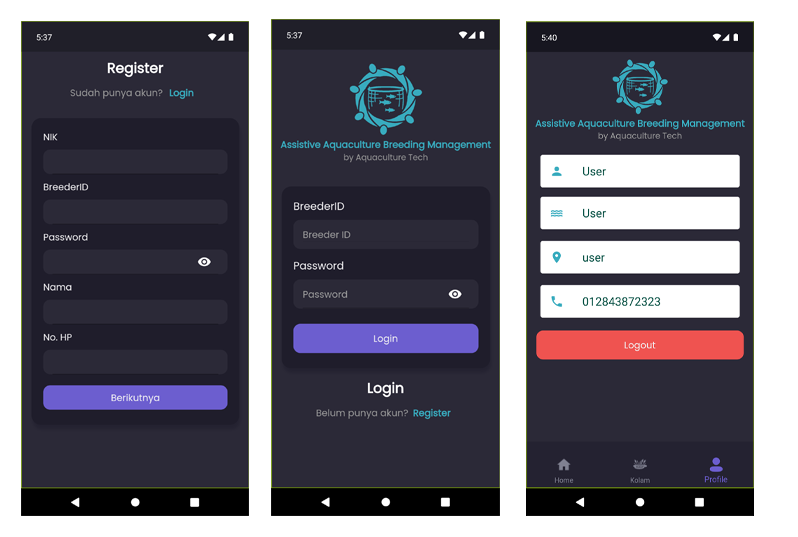
\includegraphics[keepaspectratio, width=8cm]{gambar/sssprint11}
		\caption{\textit{Output dari code pada sprint 11}}
		\label{gambar:sssprint11}
		\end{figure}

	\item{\textit{Mengitegrasikan fitur multiuser dengan webservice}}

    Hal yang dilakukan dalam mengintegrasikan fitur multiuser dengan webservice terpadat pada lampiran 12.

    \item{Analisis \textit{User Experience}} 
 
    Pada halaman register, pembudidaya harus memasukan data yang diperlukan untuk melakukan register sesuai dengan kesepakatan saat meeting. Setelah melakukan pendaftaran/register user dapat melakukan login dengan akun yang telah didaftarkan dengan menggunakan breeder ID dan password. Terdapat pula halaman profile yang berisi informasi yang terkait akun user/pembudidaya, dihalaman tersebut user dapat melakukan logout.
  

\item{Sprint 11 Review}

Sprint 11 diakhiri dengan melakukan weekly meeting pada hari selasa dengan agenda melakukan review dan testing terkait hasil sprint 11 dan melakukan planning untuk testing keseluruhan dengan rincian:
\begin{enumerate}
	\item{\textit{Review dan Testing hasil dari sprint 11}}

  Telah dilakukan review dan testing oleh penulis selaku developer dengan Scrum Master. Setelah dilakukan testing, Scrum Master menyimpulkan bahwa fitur multiuser telah berjalan dengan baik.

  \begin{longtable}{| p{8cm} | c | c | l |}
    \caption{Unit testing Halaman Awal.\label{table:unit_testing_fitur_awal}}\\
    \hline
    \multirow{2}{*}{Skenario Pengujian} & \multicolumn{2}{l|}{Kesesuaian} & \multirow{2}{*}{Kesimpulan} \\ 
    \cline{2-3}
      & \multicolumn{1}{l|}{sesuai} & tidak sesuai & \\ 
    \hline
    \hline
    \endfirsthead
    \hline
    \multirow{2}{*}{Skenario Pengujian} & \multicolumn{2}{l|}{Kesesuaian} & \multirow{2}{*}{Kesimpulan} \\ 
    \cline{2-3}
      & \multicolumn{1}{l|}{sesuai} & tidak sesuai &  \\ 
    \hline
    \hline
    \endhead
    \hline
    \endfoot
    
    
    \hline\hline
    \endlastfoot
    Saat aplikasi dibuka akan muncul splash screen yang menampilkan logo yang menandakan aplikasi sedang loading & \Checkmark &  & Diterima \\ 
    \hline
    Setelah loading selesai maka akan ditampikan halaman login & \Checkmark & & Diterima \\ 
    \hline
    \end{longtable}
    
    
    \begin{longtable}{| p{8cm} | c | c | l |}
    \caption{Unit testing Halaman Login.\label{table:unit_testing_fitur_login}}\\
    \hline
    \multirow{2}{*}{Skenario Pengujian} & \multicolumn{2}{l|}{Kesesuaian} & \multirow{2}{*}{Kesimpulan} \\ 
    \cline{2-3}
      & \multicolumn{1}{l|}{sesuai} & tidak sesuai & \\ 
    \hline
    \hline
    \endfirsthead
    \hline
    \multirow{2}{*}{Skenario Pengujian} & \multicolumn{2}{l|}{Kesesuaian} & \multirow{2}{*}{Kesimpulan} \\ 
    \cline{2-3}
      & \multicolumn{1}{l|}{sesuai} & tidak sesuai &  \\ 
    \hline
    \hline
    \endhead
    \hline
    \endfoot
    
    
    \hline\hline
    \endlastfoot
     Ketika mengisi form login dengan data yang sesuai kemudian menekan submit, maka akan masuk ke halaman dashboard & \Checkmark &  & Diterima \\ 
    \hline
     Ketika mengisi form login dengan data yang tidak sesuai kemudian menekan submit, maka akan menampilkan pesan kesalahan & \Checkmark & & Diterima \\ 
    \hline
    \end{longtable}
\end{enumerate}
\end{enumerate}